%% V1.0
%% by Gabriel Garcia, gabrcg@gmail.com
%% This is a template for Udacity projects using IEEEtran.cls

%% Be Udacious!

\documentclass[10pt,journal,compsoc]{IEEEtran}

\usepackage[pdftex]{graphicx}    
\usepackage{cite}
\hyphenation{op-tical net-works semi-conduc-tor}


\begin{document}

\title{Deep Reinforcement Learning for Robot Arm Manipulation}

\author{Deepak Trivedi}

\markboth{Deep Reinforcement Learning, DQN, Robotics, ROS}%
{}
\IEEEtitleabstractindextext{%

\begin{abstract}
Effective use of deep Q-learning is demonstrated using a robotic manipulator. The manipulator is trained using suitable rewards and punishments in order for its end effector (gripper) to come into contact with a cylindrical object. The benefit of this approach is that it does not require building a model of the manipulator or the environment. Q-learning can handle problems with stochastic transitions and rewards, without requiring adaptations.

\end{abstract}

% Note that keywords are not normally used for peerreview papers.
\begin{IEEEkeywords}
Robot,  Deep Reinforcement Learning, DQN
\end{IEEEkeywords}}


\maketitle
\IEEEdisplaynontitleabstractindextext
\IEEEpeerreviewmaketitle
\section{Introduction}
\label{sec:introduction}


\IEEEPARstart{Q}{-learning} is a reinforcement learning technique that technique does not require a model of the environment. Another benefit of Q-learning is that it can also handle problems with stochastic transitions and rewards, without requiring adaptations \cite{WikipediaQlearning}. Deep Q-learning combines with reinforcement learning a deep convolutional neural network. Layers of tiled convolutional filters mimic the effects of receptive fields. 

The DQN technique uses experience replay, a biologically inspired mechanism that uses a random sample of prior actions instead of the most recent action to proceed. This removes correlations in the observation sequence and smoothing changes in the data distribution. Iterative update adjusts Q towards target values that are only periodically updated, further reducing correlations with the target. \cite{WikipediaQlearning}

Nvidia provides an open source platform called “jetson-reinforcement” that could be integrated with Gazebo to implement DQN on robotic agents. Gazebo is an open source robotics simulator that allows realistic simulation of robots that could be controlled. 

In this project, the jetson-reinforcement platform is used to implement DQN on a robotic manipulator. There are two tasks that the robot should be able to perform. 

* Task 1: Any part of the robot arm should touch the cylindrical object with at least 90\% accuracy for a minimum of 100 episodes.
* Task 2: The gripper base of the robot arm should touch the cylinder with at least 80\% accuracy for a minimum of 100 episodes. If any other part of the arm touches the cylinder, the robot has failed and the episode is over.

In both tasks, if the robotic arm touches the ground, the robot fails and the episode is over.


%example for inserting image
%\begin{figure}[thpb]
%      \centering
%      \includegraphics[width=\linewidth]{Rudolf_Kalman.jpg}
%      \caption{Rudolf Kalman 1930-2016 \cite{Kalmanpic}, of Kalman filter fame.}
%      \label{fig:robot1}
%\end{figure}


\section{Background}

Deep Reiforcmeent Learning was first described in a 2015 paper published in Nature \cite{Naturepaper}. The authors describe  a Deep Reinforcmeent Learning system which combines Deep Neural Networks with Reinforcement Learning,  and is able to master a diverse range of Atari 2600 games to superhuman level with only the raw pixels and score as inputs \cite{Deepmind}. This is a powerful idea because of its generality. The algorithm makes it unnecessary to create separate algorithms to do a wide variety of tasks. This work represents the first demonstration of a general-purpose agent that is able to continually adapt its behavior without any human intervention, a major technical step forward in the quest for general AI \cite{Deepmind}.



\section{DQN Agent Parameters}
Successful convergence of the DQN agent depends on fine tuning of various parameters. For the purpose of this project, this notably includes the reward functions and the hyperparameters that governs the reinforcement learning and aspects of the deep neural network. In this section, the choice of these parameters will be explained. 

% Robot Models


\subsection{Model hyperparameters}

Table 1 describes the model hyperparameters, including the values chosen. The rationale for picking these values is also briefly noted. 

\begin{table*}[ht]
\caption{Model hyperparameters for the DQN agent.}
\centering
\begin{tabular}{p{0.2\linewidth}p{0.15\linewidth}p{0.15\linewidth}p{0.35\linewidth}}
\hline
Parameter & Value for Task 1  & Value for Task 2 & Notes\\
\hline
VELOCITY\_CONTROL & false & false & Displacement control was found to be more effective. Displacement control means the joint angles are controlled, while velocity control means joint velocities are controlled.  \\
INPUT\_CHANNELS & 3 & 3 & This refers to the number of channels in the input images. The three channels are red, green and blue\\
NUM\_ACTIONS & 6 & 6 & This is twice the number of degrees of freedom of the manipulator.\\
ALLOW\_RANDOM & true & true & This means that the DQN agent is allowed to take random actions. This is necessary so that the agent can explore the environment and stumble upon better rewards.\\
DEBUG\_DQN & true & true & This flag allows details such as collisions and rewards to be output to the console for debugging. \\
GAMMA & 0.9f & 0.9f & \\
EPS\_START & 0.9f & 0.9f & The probability of choosing a random action will start at EPS\_START and will decay exponentially towards EPS\_END. EPS\_DECAY controls the rate of the decay.\\
EPS\_END & 0.05f & 0.05f & See above. Larger numbers were tried too. Larger numbers helps more exploration but reduces final accuracy. \\
EPS\_DECAY & 200 & 200 & See above.\\
INPUT\_WIDTH  & 64 & 64 & Width/Height of the image used as input to the convolutional neural network. Larger resolution slows down computation. Too coarse a resolution affects accuracy. 64 worked very well.\\
INPUT\_HEIGHT & 64 & 64 & See above\\
OPTIMIZER & "RMSProp" & "Adam" & Optimizer to use for the neural network. The other option tried was RMSProp. It converged slower.\\
LEARNING\_RATE & 0.05f & 0.05f & Learning rate for the above algorithm. Values from 0.01 to 0.1 were tried. Larger values were detrimental to getting a good final accuracy.\\
REPLAY\_MEMORY & 10000 & 20000 & Memory size for experience replay, a random sample of prior actions instead of the most recent action to proceed. \\
BATCH\_SIZE & 8 & 256 & Batch size for optimization. Smaller batch size affected convergence stability. Larger batch size made the process very slow. For initial tests, a much smaller size (4 to 16) was used and it was graduall increased when other parameters were tuned.\\
USE\_LSTM & true & true & Long Short Term Memory. This was always used so that the Recurrent Neural Networks makes good use of the entire sequence of actions in order to learn what policies work.\\
LSTM\_SIZE & 256 & 256 & Size of the LSTM\\
REWARD\_WIN & 100.0f & 30000.0f & Parameter that determines the reward given to the agent if it achieves the goal.\\
REWARD\_LOSS & -100.0f & -30000.0f & Parameter that determines the reward given to the agent if it fails to achieve the goal.\\
\hline
\end{tabular}
\end{table*}

\subsection{Reward functions}

Choosing appropriate reward function was a delicate task for this project since there was often a thin line dividing failure and success. Strict punishment for failure could discourage the robot from trying. A lot of trial and error was involved in coming up with functions that finally worked. Determining how effective the functions are was difficult at times because of the stochastic nature of the learning process. The final set of reward functions that worked are described in Table 2. 


\begin{table*}[ht]
\caption{Rewards for the DQN agent.}
\centering
\begin{tabular}{p{0.2\linewidth}p{0.1\linewidth}p{0.25\linewidth}p{0.3\linewidth}}
\hline
Condition & Task 1  & Task 2 & Notes\\
\hline
Arm touches ground & -100 & -30000 & Reward for failure.  \\
Arm (excluding gripper base) touches cylinder & +100 & -30000 & This is success for Task 1 but failure for Task 2\\
Gripper base touches cylinder & 100 & +30000 + 50*number of runs remaining & Rewarding the robot for reaching the goal quickly. \\
Episode ends inconclusively & -100 & -30000 & Not getting anywhere is failure.\\
Interim rewards & avgGoalDelta & 500*int(avgGoalDelta>0.01) + int(avgGoalDelta>0.01)* (200/(0.01+distGoal)- 150/(0.01+distArm) + 150/(0.01+distHorizGoal))  & A combination of total and horizontal distance of gripper from the goal, penalizing stalled arm, and penalizing arm getting close to cylinder. Please see code for more details \\
Arm stalls & N/A & if (abs(avgGoalDelta)<0.005) rewardHistory -=500; & Punish arm if it doesn't move much in any direction\\ 
Arm moves too far way & N/A & if (distGoal>1.75) rewardHistory -=2000; & Discourage arm going in a totally wrong direction \\
\hline
\end{tabular}
\end{table*}

\section{Results}

With appropriate rewards, hyperparameters and training, the DQN agent was able to accomplish both tasks. 

Figure \ref{fig:task1} shows a screenshot of the simulation environment taken during training for Task 1. It can be seen that the DQN algorithm achieves an accuracy of more than 90\% for more than 100 iterations. In fact, the accuracy is near 100\% after about 50 iterations. 


\begin{figure*}[thpb]
      \centering
      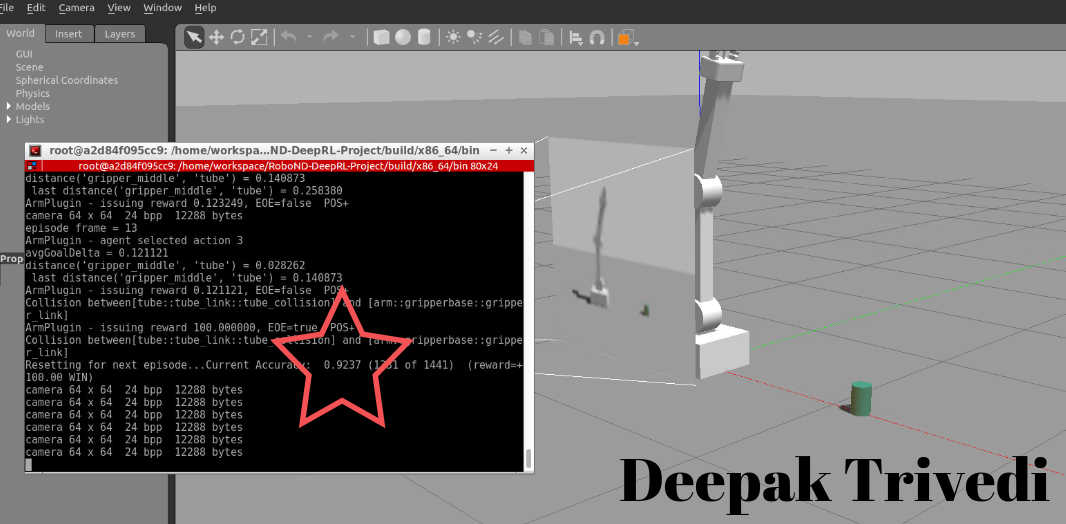
\includegraphics[width=\linewidth]{Task1.png}
      \caption{A screenshot taken during the training of Task 1 showing an accuracy of more than 90\% for more than 100 iterations }
      \label{fig:task1}
\end{figure*}

Figure \ref{fig:task2} shows a screenshot of the simulation environment taken during training for Task 2. It can be seen that the DQN algorithm achieves an accuracy of more than 80\% for more than 100 iterations. Just like in Task 1, accuracy keeps increasing gradually over time. 

It was discovered that it is important to have a good start. Because of stochastic nature of the method, if there are no early successes, the DQN agent gets lost. In this case, it is appropriate to restart until a good start is achieved. 

\begin{figure*}[thpb]
      \centering
      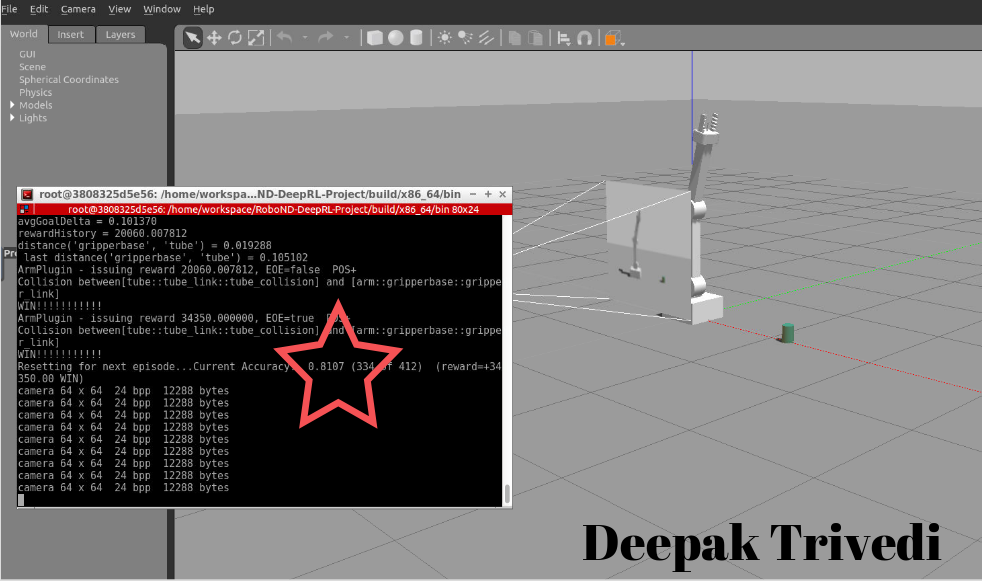
\includegraphics[width=\linewidth]{Task2.png}
      \caption{A screenshot taken during the training of Task 2 showing an accuracy of more than 80\% for more than 100 iterations }
      \label{fig:task2}
\end{figure*}

Videos for both the Tasks are available at \cite{Youtube1} and \cite{Youtube2}. 
\section{Discussion / Future work}

Several lessons were learned from this project that are worth mentioning. First, it was learned that developing appropriate reward functions could be in itself a delicate task, on the edge of being an art. It is difficult to immediately quantify the effect of various changes made in the parameters or rewards because of the stochastic nature of the algorithm. Therefore, deployment of this method may only be suitable where traditional methods such as physics-based modeling are prohibitively complicated. However, with more experience with the process it may become possible to come up with rewards and hyperparameters more easily. 

Several challenging extensions of the project were suggested, such as those involving an additional degree of freedom. These would be interesting to try. 
With a few additional steps, it should be possible to deploy the solution on hardware. For example, a Jetson TX2 could be used to control motor drivers and interface with a camera. Given fewer time constraints, it would be interesting to deploy this on a Jetson TX2. 


\bibliography{bib}
\bibliographystyle{ieeetr}

\end{document}
